\documentclass{article}%
\usepackage[T1]{fontenc}%
\usepackage[utf8]{inputenc}%
\usepackage{lmodern}%
\usepackage{textcomp}%
\usepackage{lastpage}%
\usepackage[head=40pt,margin=0.5in,bottom=0.6in]{geometry}%
\usepackage{graphicx}%
%
\title{\textbf{Maduro anunció nuevo sueldo mínimo}}%
\author{El Nacional Web}%
\date{29/11/2018}%
%
\begin{document}%
\normalsize%
\maketitle%
\textbf{URL: }%
http://www.el{-}nacional.com/noticias/politica/maduro{-}anuncio{-}nuevo{-}sueldo{-}minimo\_260501\newline%
%
\textbf{Periodico: }%
EN, %
ID: %
260501, %
Seccion: %
Política\newline%
%
\textbf{Palabras Claves: }%
NO\_TIENE\newline%
%
\textbf{Derecho: }%
2.3, %
Otros Derechos: %
, %
Sub Derechos: %
2.3.5\newline%
%
\textbf{EP: }%
NO\newline%
\newline%
%
\textbf{\textit{El mandatario indicó que el nuevo salario se establecerá en diciembre}}%
\newline%
\newline%
%
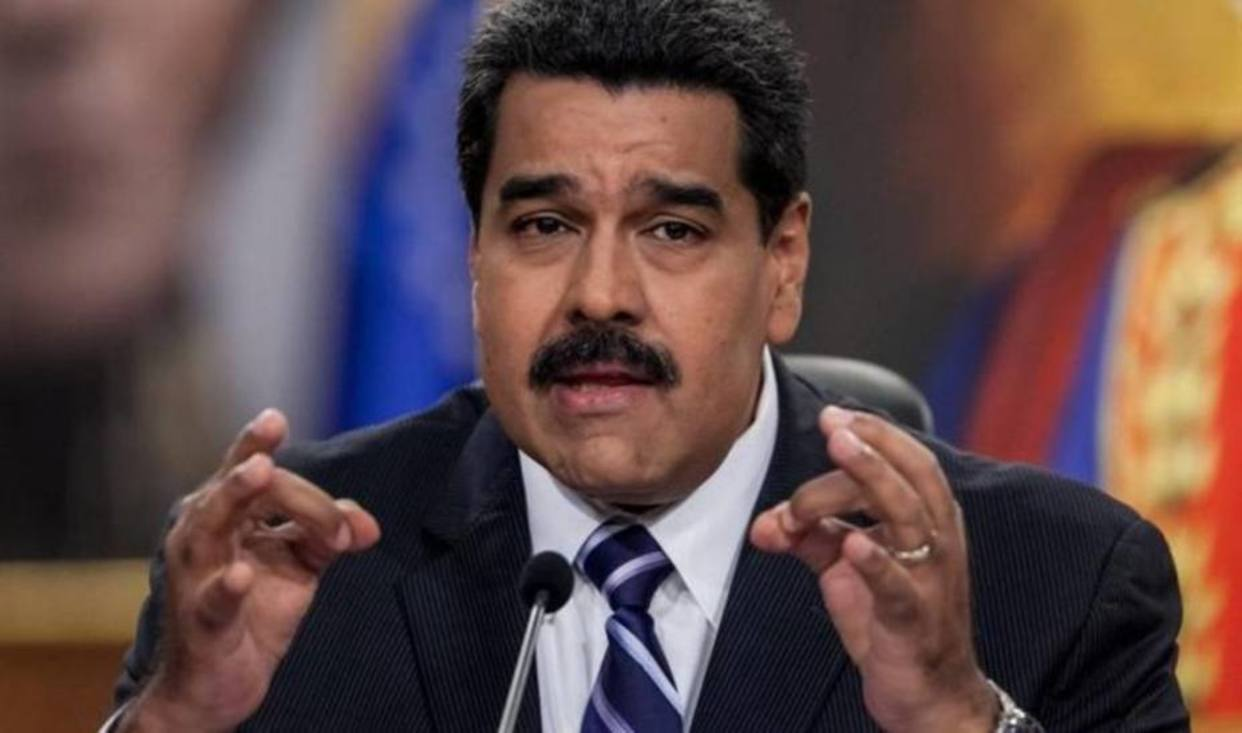
\includegraphics[width=300px]{261.jpg}%
\newline%
%
El presidente Nicolás Maduro anunció este jueves, durante su reunión con el gabinete económico,~que el nuevo salario mínimo es de 4.500 bolívares.%
\newline%
%
“Lo que estamos haciendo no está en ningún manual de economía. Tenemos equipos de primer nivel que nos están asesorando con propuestas para lograr nuestros ~objetivos”, afirmó Maduro.%
\newline%
%
El incremento, que~fue anunciado,~durante una transmisión conjunta de radio y televisión, ocurre a tres meses~de la activación del "programa de recuperación económica, crecimiento y prosperidad".%
\newline%
%
El nuevo sueldo regirá a partir del primero de diciembre, y supone 150\% de incremento en relación con el monto anterior.%
\newline%
%
\end{document}